\documentclass[fleqn]{article}
\usepackage{fullpage}
\usepackage{amsmath}
\usepackage{enumitem}
\usepackage{amssymb}
\usepackage{listings}
\usepackage{hyperref}
\usepackage{tikz}
\usepackage{algpseudocode}
\usepackage{algorithm}
\usepackage{multicol}

\renewcommand{\vec}[1]{\mathbf{#1}}

\DeclareMathOperator*{\argmax}{arg\,max}
\usetikzlibrary{arrows}
\lstset{basicstyle=\ttfamily, mathescape}
\graphicspath{{./img/}}

\usepackage[utf8]{inputenc}

% Default fixed font does not support bold face
\DeclareFixedFont{\ttb}{T1}{txtt}{bx}{n}{12} % for bold
\DeclareFixedFont{\ttm}{T1}{txtt}{m}{n}{12}  % for normal

% Custom colors
\usepackage{color}
\definecolor{deepblue}{rgb}{0,0,0.5}
\definecolor{deepred}{rgb}{0.6,0,0}
\definecolor{deepgreen}{rgb}{0,0.5,0}

\usepackage{listings}

% Python style for highlighting
\newcommand\pythonstyle{\lstset{
language=Python,
basicstyle=\tt,
otherkeywords={self},             % Add keywords here
keywordstyle=\tt\color{deepblue},
emph={MyClass,__init__},          % Custom highlighting
emphstyle=\tt\color{deepred},    % Custom highlighting style
stringstyle=\color{deepgreen},
frame=tb,                         % Any extra options here
showstringspaces=false            %
}}


% Python environment
\lstnewenvironment{python}[1][]
{
\pythonstyle
\lstset{#1}
}
{}

% Python for external files
\newcommand\pythonexternal[2][]{{
\pythonstyle
\lstinputlisting[#1]{#2}}}

% Python for inline
\newcommand\pythoninline[1]{{\pythonstyle\lstinline!#1!}}

\title{\textbf{Preliminary Report - Edibility of Mushroom Species}}
\author{
    \begin{tabular}{cccc}
            Ishaan Saxena      & Nikita Rajaneesh    & Swaraj Bhaduri     & Utkarsh Jain       \\
            isaxena@purdue.edu & nrajanee@purdue.edu & sbhadur@purdue.edu & jain192@purdue.edu
    \end{tabular}
}

% Document
\begin{document}
    \maketitle

    % 1
    \section{Introduction to the Problem}

    % 1.1
    \subsection{Definition of the Problem}

    Given a dataset $ \mathcal{D} $ with $ n=8124 $ samples where each sample represents a
    mushroom with features being the observations about the characterestics of the mushrooms
    such as odor, color, etc., we aim to test and compare various supervised learning models
    for the problem of classifying each sample into either poisonous or edible. Further,
    we will optimize the Hyperparameters of the model which initially performs the best
    on the dataset.\footnote{This dataset can be found at
    \href{https://www.kaggle.com/uciml/mushroom-classification}
    {https://www.kaggle.com/uciml/mushroom-classification}.}

    % 1.2
    \subsection{Data Description}

    We are given $ \mathcal{D} $ with $ n=8124 $ samples wherein each sample has the
    following 22 features (excluding the class label).

    \begin{multicols}{3}
        \begin{enumerate}
            \item cap-shape
            \item cap-surface
            \item cap-color
            \item bruises
            \item odor
            \item gill-attachment
            \item gill-color
            \item stalk-root
            \item stalk-surface-above-ring
            \item stalk-surface-below-ring
            \item stalk-color-above-ring
            \item stalk-color-below-ring
            \item veil-type
            \item veil-color
            \item ring-type
            \item spore-print-color
            \item habitat
            \item gill-spacing
            \item gill-size
            \item stalk-shape
            \item ring-number
            \item population
        \end{enumerate}
    \end{multicols}
    \noindent
    These features have been further enumerated in Appendix A.

    % 1.3
    \subsection{Encoding the Data}

    Note that all the features in our dataset are categorical variables. As a result, to
    proceed with evaluation of model performance, we must first encode these variables
    into numerical/binary values.\\

    We need to deal with two kinds of categorical variables when encoding the features
    into numerical data. These are ordinal categorical variables and nominal categorical
    variables.\footnote{Information on which features are which kind of categorical
    variables can be found in Appendix A.} We will use different techniques to encode
    both of these kinds of categorical variables as they inherently represent different
    kinds of categorical data.

    \subsubsection{Nominal Categorical Variables}

    To encode nominal categorical variables, we will use one-hot binary features. For
    instance, if a feature $ f $ from a feature set $ \mathcal{F} $ has $ k $ different
    categorical values, we can create $ k $ different binary features for each feature
    $ f $ of this kind. This is done because the values of each such feature do not hold
    any ordinal information, in that there should not be different weights for having a
    specific value of a specific feature.

    \subsubsection{Ordinal Categorical Variables}

    The ordinal categorical variables, on the other hand, have been encoded as numerical
    labels, as these informations contain valueable information about the 'scale' of a
    certain feature. For instance, if a feature $ f $ from a feature set $ \mathcal{F} $
    has $ k $ different features, it would be changed into numeric values
    $ i \in 0,1,...,k-1$.

    \subsubsection{Encoding Process}

    The following code segment is used to encode the data.\footnote{This can be found in
    the data.py file.}

    \begin{python}
def encode(df):
    # Encode Ordinal Variables
    ordinal_columns = ['gill-spacing', 'gill-size',
            'stalk-shape', 'ring-number', 'population', 'class']
    columns = ordinal_columns[:]

    for column in columns:
        df[column] = df[column].astype('category')

        columns = df.select_dtypes(['category']).columns
        df[columns] = df[columns].apply(lambda x: x.cat.codes)

    # Encoding Nominal Variables
    columns = ordinal_columns[:]

    for column in df:
        if column not in columns:
            dummies = pd.get_dummies(df.pop(column))
            column_names = [column + "_" + x for x in dummies.columns]
            dummies.columns = column_names
            df = df.join(dummies)

    return df
    \end{python}

    \noindent
    We can now see how our encoded dataset $ \mathcal{D} $ is shaped, and then proceed
    further in our task to classify data.

    \begin{python}
>>> X, y = data.load() # data.load() calls data.encode()
>>> X.shape
(8124, 107)
>>> y.shape
(8124,)
    \end{python}

    % 2
    \section{Feature Selection}

    % 2.1
    \subsection{The Need for Feature Selection}
    Feature selection is a useful technique when we want to better understand the input
    feature set. Having fewer features also leads to a more interpretable model, and is
    definitely helpful in our case, since we have just created over 100 features from
    which we want to derive a model to solve the classification problem. As a result,
    feature selection techniques can help us get a better idea of which features matter
    more or less while classifying our model.\\

    It is also important to note that feature selection helps us have a control over the
    complexity of the model. This is a very important aspect, as a less complex model
    is more useful for generalization.

    % 2.2
    \subsection{Feature Selection Technique}
    We are using Greedy Subset Selection for Feature Selection. We will talk more about
    the selection technique and its implementation in the final report.

    % 2.3
    \subsection{Greedy Subset Selection Results}
    The following are the 46 best features and their weights obtained from Greedy Subset
    Selection:

    \begin{center}
        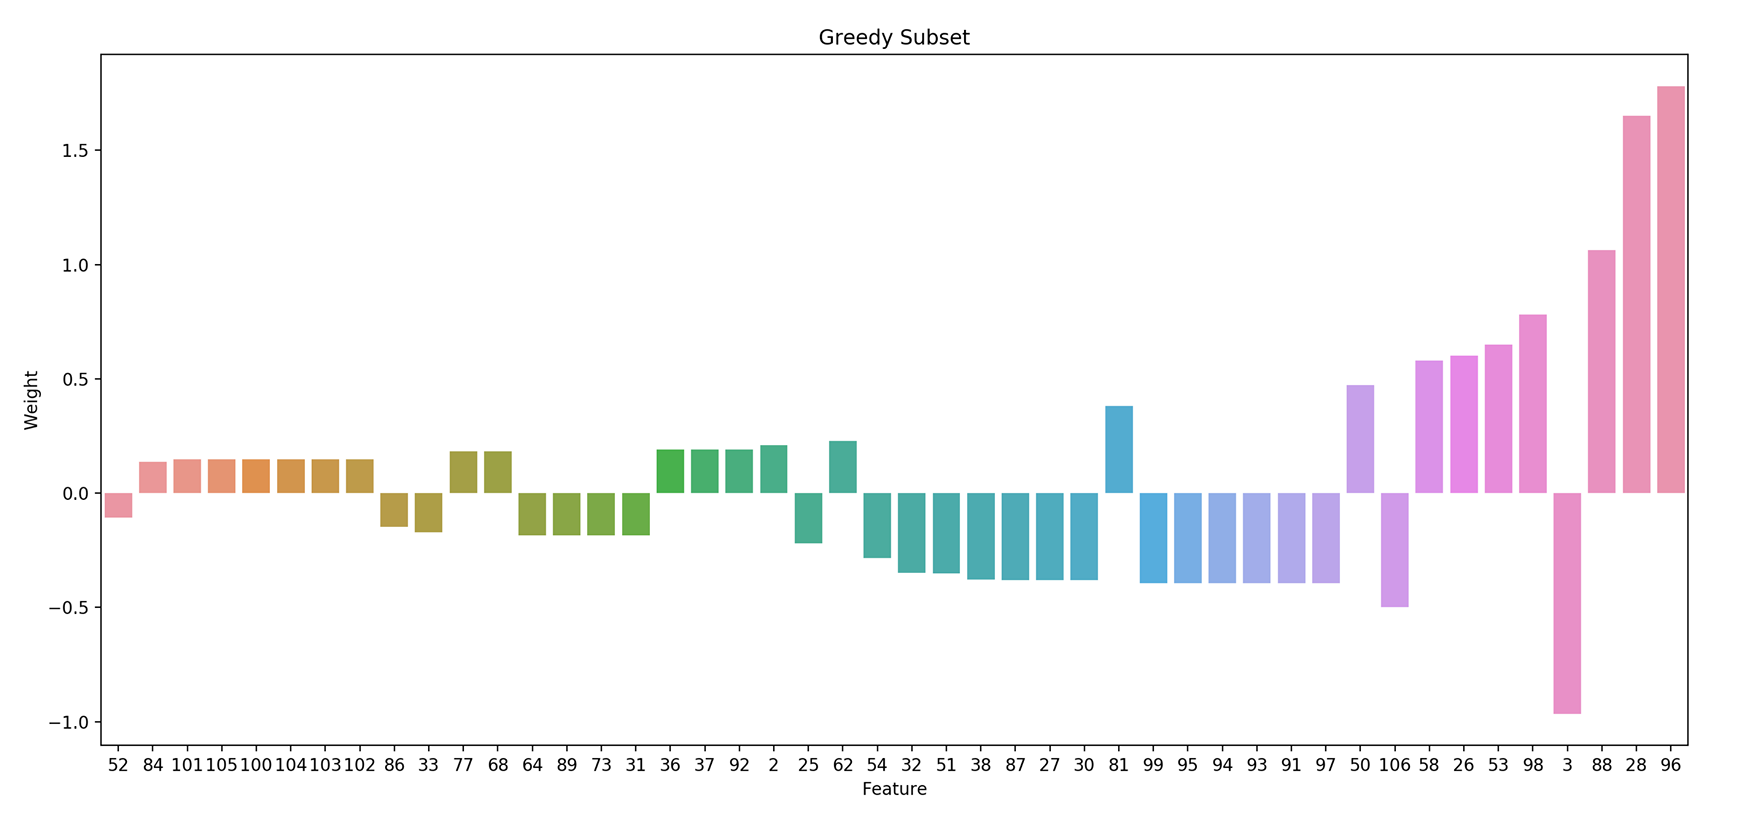
\includegraphics[scale=0.27]{46.png}
        \begin{figure}[!h]
            \caption{Greedy Subset Selection - 46 features with highest weights.}
        \end{figure}
    \end{center}


    We will talk more about reduction of features, how that impacts our problem,
    and about what these specific features are in the final report.

    % 3
    \section{Machine Learning Models}

    In order to solve the classification problem,
    % with a reduced number of features,
    we will test the following machine learning algorithms with $ \{2, 5, 10\} $-Fold Cross
    Validation and different metrics, including Hypothesis Testing, ROC Curves, etc.
    to compare the results:
    \begin{enumerate}
        \item Perceptron
        \item Support Vector Machine
        \item Logistic Regression
        \item Adaboost
    \end{enumerate}

    \subsection{Cross-Validation Technique: $k$-Fold CV}
    We use cross-validation to evaluate the chosen predictive model by paritioning it into
    smaller train and test datasets wherein we train the model on the training set and
    evaluate it on the testing set. By using better cross-validation techniques, we can
    get a better understanding of how well our model will generalize, and whether we might
    be over or underfitting.\\

    Here, we are using $k$-Fold Cross Validation on 2, 5, and 10 folds. In $k$-Fold CV, we
    split the dataset into $k$ different folds. For each $i^{th}$ fold, where
    $ i = 1, 2,...,k $, we train on the remaining $ k-1 $ folds and evaluate on the single
    remaining fold. As a result, we get $ k $ different measures of the metrics which we
    are using for each model we evaluate using the cross-validation technique. These can
    be aggregated into a single metric as follows:

    $$  \hat\mu = \frac{1}{k} \sum_{1\leq i \leq k} M_i \text{, and }
        \hat\sigma^2 = \frac{1}{k} \sum_{1\leq i \leq k} (M_i - \hat\mu)^2 $$

    \noindent
    where $ M_i $ is the measure for the $i^{th}$ fold (here, it is accuracy). This
    aggregation may be used in a statistical hypothesis test to compare the performances
    of two different models.\\

    \noindent
    The following is our implementation of $k$-fold cross validation:\footnote{This can be
    found in the kfoldcv.py file.}

    \begin{python}
    # For each fold
    for i in range(k):
        # Find sets S and T
        lower = np.floor(float(n) * i / k).astype('int64')
        upper = np.floor(float(n) * (i + 1) / k - 1).astype('int64')
        T = range(lower, upper + 1)
        S = list(range(0, lower)) + list(range(upper + 1, n))

        # Get training data
        X_train = X[S, :]
        y_train = y[S]

        # Fit model
        m = model(**kwargs)
        m.fit(X_train, y_train)

        # Check prediction accuracy
        y_pred = m.predict(X[T])

        # Update Z values based on accuracy score
        Z[i] = metrics.accuracy_score(y[T], y_pred)

    # Return k-Fold results
    return Z
    \end{python}

    \noindent
    To see how this we utilize this script to get results for specific models, please see
    Appendix B.

    \subsection{Model $k$-Fold CV Results}
    \subsubsection{Perceptron}
    \begin{center}
        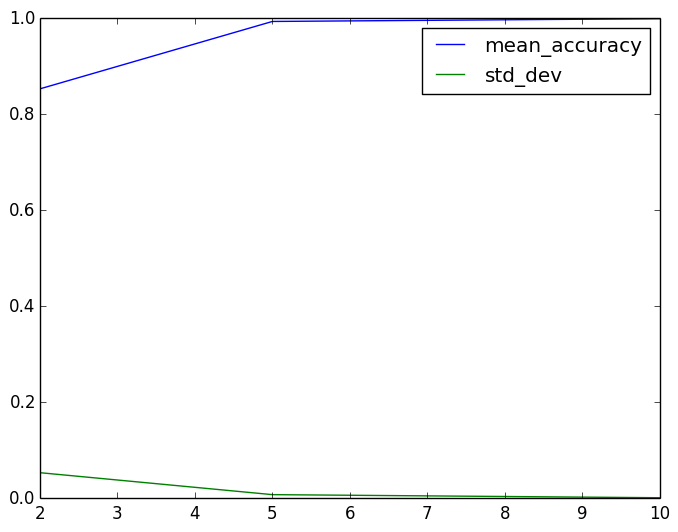
\includegraphics[scale=0.35]{model_accuracy_vs_folds_Perceptron.png}
        \begin{figure}[!h]
            \caption{Perceptron accuracy in 2,3,5-Fold CV}
        \end{figure}
    \end{center}
    We get the following results for a Perceptron when we run kfoldcv\_graph.py:
    \begin{lstlisting}
    Model: Perceptron
        2-fold: (mu=0.853, sigma=0.054)
        5-fold: (mu=0.994, sigma=0.008)
        10-fold: (mu=1.000, sigma=0.001)
        Time: 9.351s
    \end{lstlisting}

    \subsubsection{SVM}
    \begin{center}
        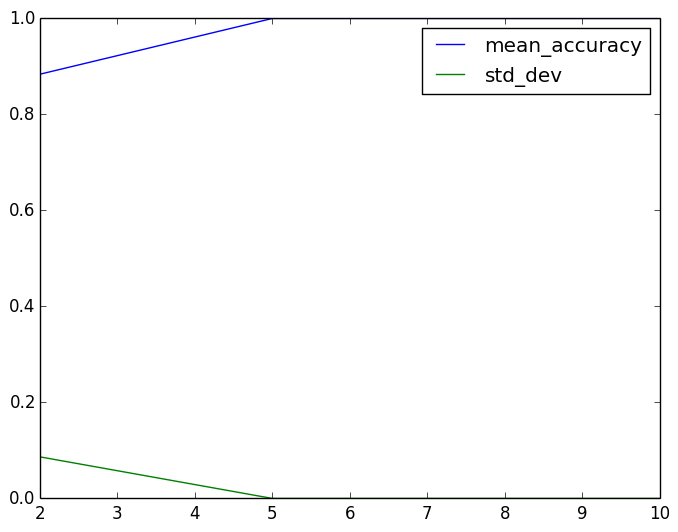
\includegraphics[scale=0.3]{model_accuracy_vs_folds_SVM-linear.png}
        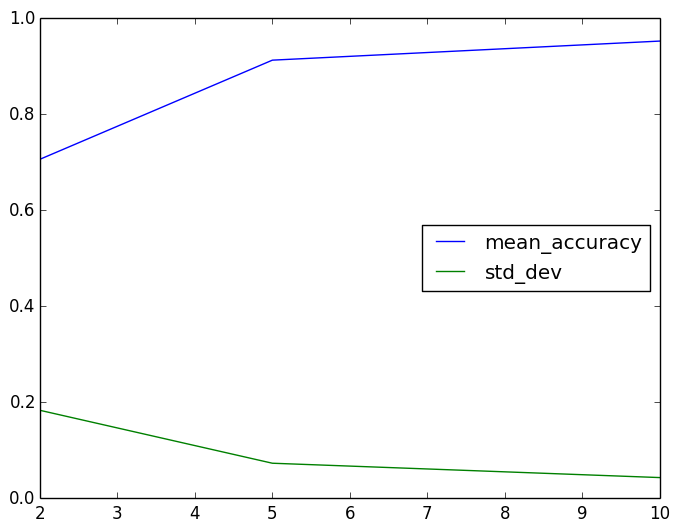
\includegraphics[scale=0.3]{model_accuracy_vs_folds_SVM-poly.png}
        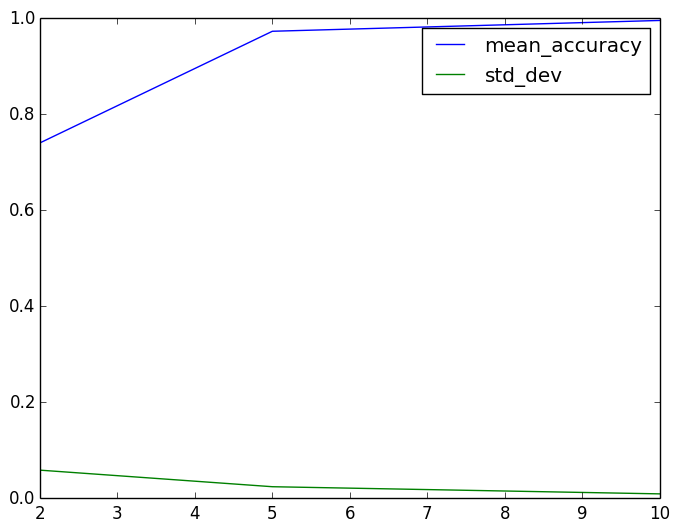
\includegraphics[scale=0.3]{model_accuracy_vs_folds_SVM-rbf.png}
        \begin{figure}[!h]
            \caption{SVM accuracy in 2,3,5-Fold CV. From left to right, we are using
            linear, polynominal, and rbf kernels.}
        \end{figure}
    \end{center}
    We get the following results for SVMs when we run kfoldcv\_graph.py:
    \begin{lstlisting}
    Model: SVM-linear
        2-fold: (mu=0.884, sigma=0.087)
        5-fold: (mu=1.000, sigma=0.000)
        10-fold: (mu=1.000, sigma=0.000)
        Time: 5.442s
    Model: SVM-poly
        2-fold: (mu=0.707, sigma=0.184)
        5-fold: (mu=0.913, sigma=0.073)
        10-fold: (mu=0.953, sigma=0.043)
        Time: 36.912s
    Model: SVM-rbf
        2-fold: (mu=0.741, sigma=0.059)
        5-fold: (mu=0.973, sigma=0.024)
        10-fold: (mu=0.996, sigma=0.010)
        Time: 13.458s
    \end{lstlisting}

    \subsubsection{Logistic Regression}
    \begin{center}
        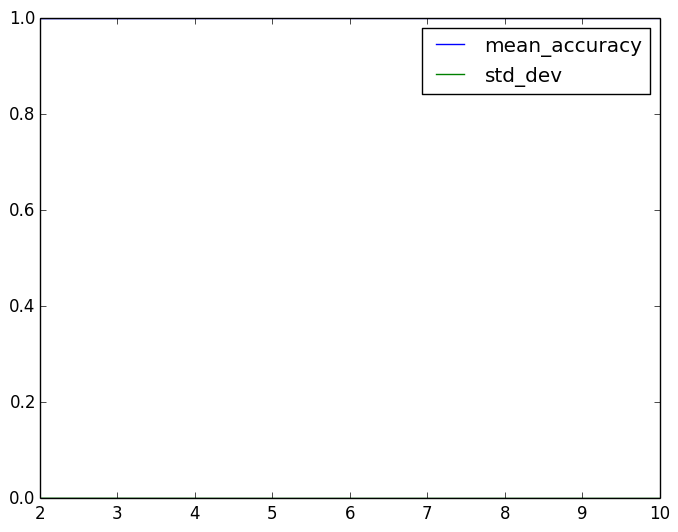
\includegraphics[scale=0.35]{model_accuracy_vs_folds_LR.png}
        \begin{figure}[!h]
            \caption{Logistic Regression accuracy in 2,3,5-Fold CV.}
        \end{figure}
    \end{center}
    We get the following results for Logistic Regression when we run kfoldcv\_graph.py:
    \begin{lstlisting}
    Model: LR
        2-fold: (mu=0.832, sigma=0.029)
        5-fold: (mu=0.986, sigma=0.014)
        10-fold: (mu=0.999, sigma=0.002)
        Time: 0.754s
    \end{lstlisting}

    \subsubsection{Adaboost}
    \begin{center}
        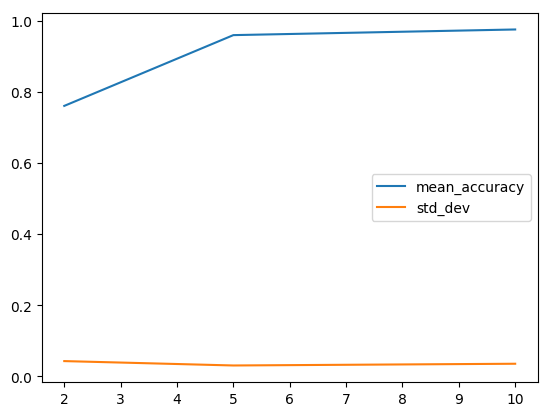
\includegraphics[scale=0.3]{model_accuracy_vs_folds_Adaboost-n_estimators10.png}
        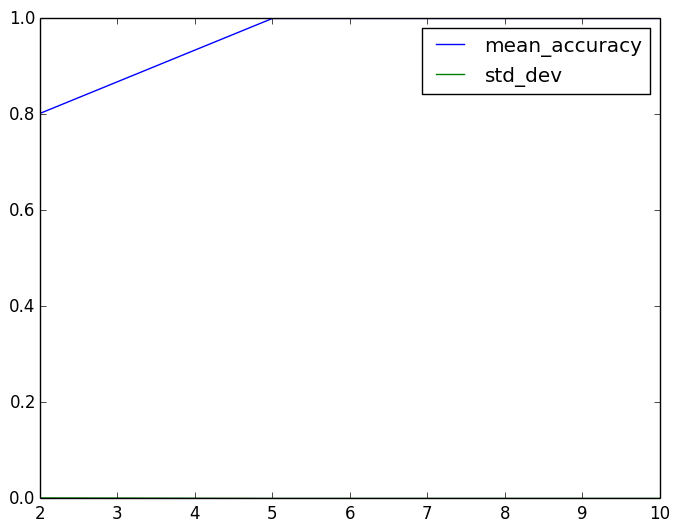
\includegraphics[scale=0.3]{model_accuracy_vs_folds_Adaboost-n_estimators50.png}
        \begin{figure}[!h]
            \caption{Adaboost accuracy in 2,3,5-Fold CV. From left to right, we have 10
            and 50 n_estimators}
        \end{figure}
    \end{center}
    We get the following results for Adaboost when we run kfoldcv\_graph.py:
    \begin{lstlisting}
    Model: Adaboost-n_estimators 10
        2-fold: (mu=0.796, sigma=0.007)
        5-fold: (mu=0.959, sigma=0.031)
        10-fold: (mu=0.975, sigma=0.035)
        Time: 1.437s
    Model: Adaboost-n_estimators 50
        2-fold: (mu=0.802, sigma=0.001)
        5-fold: (mu=1.000, sigma=0.000)
        10-fold: (mu=1.000, sigma=0.000)
        Time: 6.402s
    \end{lstlisting}

    % Appendices
    % Appendix A
    \newpage
    \section*{\underline{Appendix A: Data Description}}
    Classes: edible=e, poisonous=p (y-values)\\

    Size of dataset (before encoding): $ (n=8124, d=22) $

    Size of dataset (after encoding): $ (n=8124, d=107) $

    Attribute Information and Encoding:
    \begin{enumerate}
        \item \underline{Nominal Categorical Variables:}\\
        These variables will be encoded as binary one-hot features. As a result, each feature
        in this category would be replace by the $ k $ features in the encoded dataset if the
        feature has $ k $ possible values. These featues include:
        \begin{enumerate}[label=\roman*.]
            \item \textbf{cap-shape}:
                bell=b,
                conical=c,
                convex=x,
                flat=f,
                knobbed=k,
                sunken=s
            \item \textbf{cap-surface}:
                fibrous=f,
                grooves=g,
                scaly=y,
                smooth=s
            \item \textbf{cap-color}:
                brown=n,
                buff=b,
                cinnamon=c,
                gray=g,
                green=r,
                pink=p,
                purple=u,
                red=e,
                white=w,
                yellow=y
            \item \textbf{bruises}:
                bruises=t,
                no=f
            \item \textbf{odor}:
                almond=a,
                anise=l,
                creosote=c,
                fishy=y,
                foul=f,
                musty=m,
                none=n,
                pungent=p,
                spicy=s
            \item \textbf{gill-attachment}:
                attached=a,
                descending=d,
                free=f,
                notched=n
            \item \textbf{gill-color}:
                black=k,
                brown=n,
                buff=b,
                chocolate=h,
                gray=g,
                green=r,
                orange=o,
                pink=p,
                purple=u,
                red=e,
                white=w,
                yellow=y
            \item \textbf{stalk-root}:
                bulbous=b,
                club=c,
                cup=u,
                equal=e,
                rhizomorphs=z,
                rooted=r,
                missing=?
            \item \textbf{stalk-surface-above-ring}:
                fibrous=f,
                scaly=y,
                silky=k,
                smooth=s
            \item \textbf{stalk-surface-below-ring}:
                fibrous=f,
                scaly=y,
                silky=k,
                smooth=s
            \item \textbf{stalk-color-above-ring}:
                brown=n,
                buff=b,
                cinnamon=c,
                gray=g,
                orange=o,
                pink=p,
                red=e,
                white=w,
                yellow=y
            \item \textbf{stalk-color-below-ring}:
                brown=n,
                buff=b,
                cinnamon=c,
                gray=g,
                orange=o,
                pink=p,
                red=e,
                white=w,
                yellow=y
            \item \textbf{veil-type}:
                partial=p,
                universal=u
            \item \textbf{veil-color}:
                brown=n,
                orange=o,
                white=w,
                yellow=y
            \item \textbf{ring-type}:
                cobwebby=c,
                evanescent=e,
                flaring=f,
                large=l,
                none=n,
                pendant=p,
                sheathing=s,
                zone=z
            \item \textbf{spore-print-color}:
                black=k,
                brown=n,
                buff=b,
                chocolate=h,
                green=r,
                orange=o,
                purple=u,
                white=w,
                yellow=y
            \item \textbf{habitat}:
                grasses=g,
                leaves=l,
                meadows=m,
                paths=p,
                urban=u,
                waste=w,
                woods=d
        \end{enumerate}
        \item \underline{Ordinal Categorical Variables:}\\
        These variables will be encoded in place by encoding labels, as the data here has
        ordinal meaning to it. These variables include:
        \begin{enumerate}[label=\roman*.]
            \item \textbf{gill-spacing}:
                close=c$\to$0,
                crowded=w$\to$1,
                distant=d$\to$2
            \item \textbf{gill-size}:
                broad=b$\to$0,
                narrow=n$\to$1
            \item \textbf{stalk-shape}:
                enlarging=e$\to$0,
                tapering=t$\to$1
            \item \textbf{ring-number}:
                none=n$\to$0,
                one=o$\to$1,
                two=t$\to$2
            \item \textbf{population}:
                abundant=a$\to$0,
                clustered=c$\to$1,
                numerous=n$\to$2,
                scattered=s$\to$3,
                several=v$\to$4,
                solitary=y$\to$5
        \end{enumerate}
    \end{enumerate}

    % Appendix B
    \newpage
    \section*{\underline{Appendix B: k-Fold CV Graphs}}

    The following code an excerpt from the file kfoldcv\_graph.py. This file uses the
    kfoldcv.py module to get metrics for multiple machine learning models and saves plots
    of accuracy vs number of folds for each of the models.

    \begin{python}
# Import models. For example:
from sklearn.svm import SVC

models = []
# Add models to list. For example:
models.append(("SVM-linear", SVC, {'kernel':'linear'}))
models.append(("SVM-poly", SVC, {'kernel':'poly'}))

# For each algorithm
for name, model, kwargs in models:
    # Folds
    folds = [2, 5, 10]
    # Mean accuracy and std dev
    m = []
    s = []
    # For each fold size
    for fold_size in folds:
        Z = kfoldcv.run(X, y, model, fold_size, **kwargs)
        m.append(np.mean(Z))
        s.append(np.std(Z))
    # Plot accuracy vs. fold size
    df = pd.DataFrame({
        'mean_accuracy': m,
        'std_dev': s
    }, index = folds)
    lines = df.plot.line()
    filename = project.results + "model_accuracy_vs_folds_" + name + ".png"
    plt.savefig(filename, bbox_inches='tight')
    \end{python}
    \noindent
    This is how the output looks when this script is run:
    \begin{lstlisting}
    Model:	SVM-linear
        2-fold: (mu=0.884, sigma=0.087)
        5-fold: (mu=1.000, sigma=0.000)
        10-fold: (mu=1.000, sigma=0.000)
        Time: 4.987s
    Model:	SVM-poly
        2-fold: (mu=0.707, sigma=0.184)
        5-fold: (mu=0.913, sigma=0.073)
        10-fold: (mu=0.953, sigma=0.043)
        Time: 33.005s
    \end{lstlisting}
    \noindent
    This file also saves graphs like in section 3 for different models.

    % Appendix B
    \newpage
    \section*{\underline{Appendix C: List of Scripts}}
    The following scripts have been included with the preliminary report in the zip file:
    \begin{enumerate}
        \item data.py - Interface to load encoded data.
        \item project.py - Contains project config.
        \item kfoldcv.py - Conduct kfoldcv.
        \item kfoldcv\_graph.py - Conduct kfoldcv for multiple models and multiple values
        of $k$ and save the results.
        \item greedySubset.py - Conduct Greedy Subset Selection.
        \item featureSelection.py - Graph the results for Greedy Subset Selection.
    \end{enumerate}


\end{document}
